
\section{Struttura del File System}

\textbf{Struttura del file}: unità di archiviazione logica e raccolta di informazioni correlate.

\textbf{Il file system fornisce: }

\begin{itemize}
    \item interfaccia utente allo storage, mappando logico su fisico
    \item accesso efficiente e comodo al disco, permettendo di memorizzare, localizzare e recuperare facilmente i dati
    \item Interfaccia all'HW: il disco fornisce riscrittura in-place e accesso casuale - i trasferimenti I/O avvengono in blocchi o settori (solitamente 512 byte)
\end{itemize}

\textbf{File control block} (\textbf{FCB}) - struttura di archiviazione contenente informazioni su un file.

\textbf{Driver del dispositivo} controlla il dispositivo fisico - molte attività: un File System può essere organizzato a livelli.


\section{File System a Livelli}

\begin{figure}[h!]
    \centering
    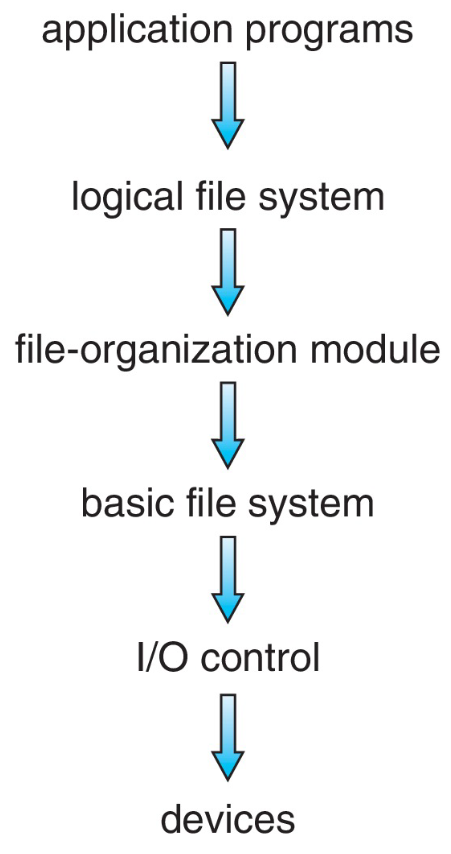
\includegraphics[width=0.25\linewidth]{content/OS_Internals/img/sdfrbn.png}
\end{figure}

\newpage
\subsection{Driver dei Dispositivi}

\textbf{I driver dei dispositivi} gestiscono i dispositivi I/O al livello di controllo I/O.


Ricevuti comandi come: leggi drive1, cilindro 72, traccia 2, settore 10, in posizione memoria 1060.


Emette comandi hardware di basso livello specifici per il controller hardware

\subsection{File System di Base}

\textbf{Il file system di base}, ricevuto un comando come “recupera blocco 123”, lo traduce in comando per il driver del dispositivo.

Gestisce anche i buffer e le cache in memoria (allocazione, liberazione, sostituzione):
\begin{itemize}
    \item I buffer contengono i dati in transito
    \item Le cache contengono i dati usati frequentemente
\end{itemize}





\subsection{Modulo di Organizzazione dei File}

\textbf{Il modulo di organizzazione} dei file comprende file, indirizzi logici e blocchi fisici.

Traduce il numero di blocco logico nel numero di blocco fisico.

Gestisce lo spazio libero e l'allocazione del disco.







\subsection{File System Logico}
Il file system logico gestisce le informazioni sui metadati:

\begin{itemize}
    \item Traduce il nome del file in numero di file, handle e posizione, mantenendo i file control block (inode in UNIX)
    \item Gestione delle directory
    \item Protezione
\end{itemize}

La stratificazione è utile per ridurre complessità e ridondanza,
ma aggiunge overhead e può diminuire le prestazioni.

I livelli logici possono essere implementati con qualsiasi metodo di codifica, a discrezione del progettista del OS.

Il file system logico viene chiamato direttamente dalle \textbf{applicazioni}, es. C open()    






\section{Tipi di File System}

Molti file system, a volte più di uno nello stesso sistema operativo, ciascuno con il proprio formato:
\begin{itemize}
    \item CD-ROM è ISO 9660;
    \item Unix ha UFS, FFS;
    \item Linux ha più di 130 tipi, con ext3 ed ext4 come estensioni del file system principale;
    \item Windows ha FAT, FAT32, NTFS oltre a floppy, CD, DVD Blu-ray.
\end{itemize}

Ne continuano ad arrivare di nuovi - ZFS, GoogleFS, Oracle ASM, FUSE

\newpage

\section{Dall'API all'Implementazione}

\subsection{Operazioni del File System}

Abbiamo system call al livello API: Open, close, read, write, seek... ma come implementiamo le loro funzioni? Mediante strutture su disco e in memoria.

\paragraph{}
\textbf{Boot control block} (o \textbf{MBR}) contiene le informazioni necessarie al sistema per avviare l'OS da quel volume. Necessario se il volume contiene l'OS, di solito il primo blocco del volume.

\textbf{Volume control block} (superblock, master file table) contiene i dettagli del volume: numero totale di blocchi, numero di blocchi liberi, dimensione del blocco, puntatori o array di blocchi liberi.

La struttura delle directory organizza i file: nomi e numeri di inode, master file table.

\subsection{Blocco di Controllo dei File - FCB}

L'OS mantiene un FCB per ogni file, che contiene molti dettagli sul file: tipicamente, numero di inode (se Linux), permessi, dimensione, date.


\begin{figure}[h!]
    \begin{minipage}[h!]{0.5\textwidth}
        \centering
        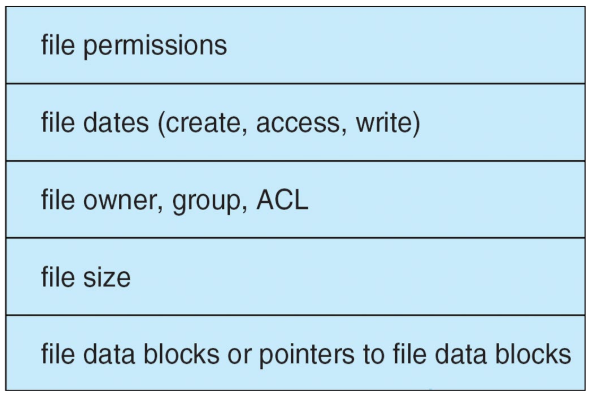
\includegraphics[width=1\linewidth]{content/OS_Internals/img/mfhg.png}
    \end{minipage}
    \begin{minipage}[h!]{0.5\textwidth}
    \centering
    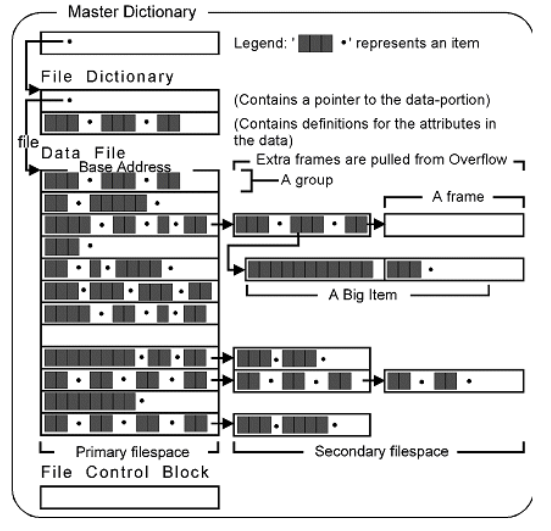
\includegraphics[width=1\linewidth]{content/OS_Internals/img/dfngb.png}     
    \end{minipage}
\end{figure}

\subsection{Il Linux iNode}

Un inode (noto anche come index node) è una struttura dati usata da Unix/Linux per descrivere un oggetto all'interno di un file system. Tale oggetto può essere un file o una directory.

Ogni inode memorizza puntatori alle posizioni dei blocchi su disco dei dati e dei metadati dell'oggetto.

In generale, i metadati contenuti in un inode sono:

\begin{itemize}
    \item tipo di file (file normale/directory/link simbolico/file speciale a blocchi/file speciale a caratteri/ecc.),
    \item permessi,
    \item ID proprietario/gruppo,
    \item dimensione,
    \item ora dell'ultimo accesso/modifica,
    \item ora di modifica dei metadati
    \item numero di hard link
\end{itemize}


\begin{figure}[h!]
    \begin{minipage}[h!]{0.5\textwidth}
        \centering
        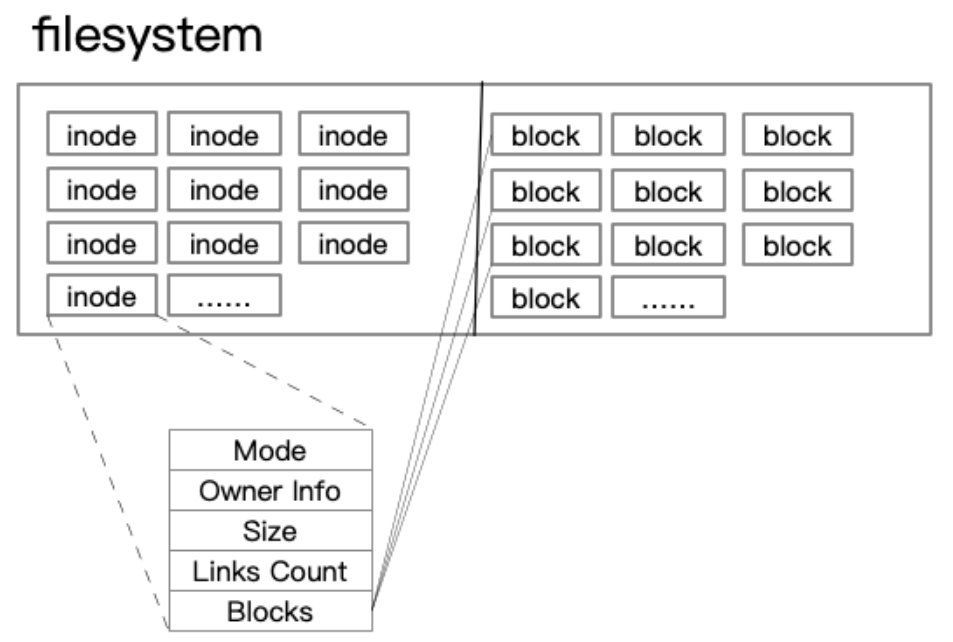
\includegraphics[width=1\linewidth]{content/OS_Internals/img/dfnsb.png}
        \caption{Il Linux iNode}
    \end{minipage}
    \begin{minipage}[h!]{0.5\textwidth}
    \centering
    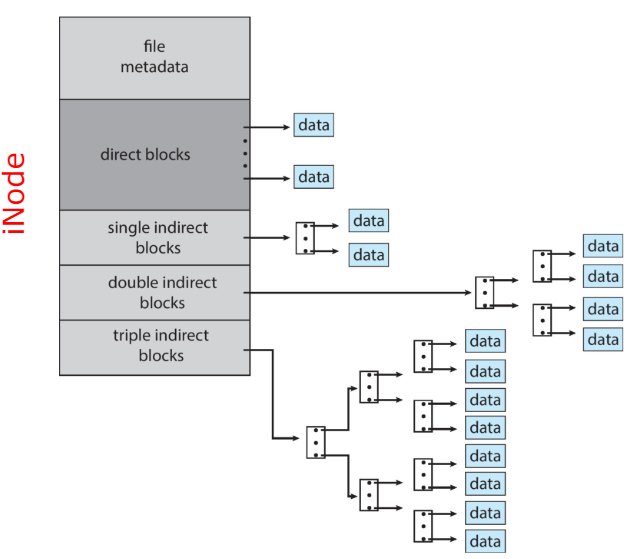
\includegraphics[width=1\linewidth]{content/OS_Internals/img/smgth.png}
    \caption{UNIX UFS - 4 KB per blocco, indirizzi a 32 bit} 
    \end{minipage}
\end{figure}


\subsection{Strutture del File System in Memoria}

\textbf{Tabella di montaggio} - memorizza i mount dei file system, i punti di montaggio e i tipi di file system.

\textbf{Tabella globale dei file aperti} - contiene una copia del FCB di ogni file e altre informazioni.

\textbf{Tabella dei file aperti per processo} - contiene puntatori alle voci appropriate nella tabella globale e altre informazioni.

\paragraph{}

Gli elementi della tabella sono chiamati:

\begin{itemize}
    \item fd descrittori di file in UNIX/Linux
    \item fh file handler in Windows
    \item stessa denominazione delle funzioni C
\end{itemize}

\begin{figure}[h!]
    \centering
    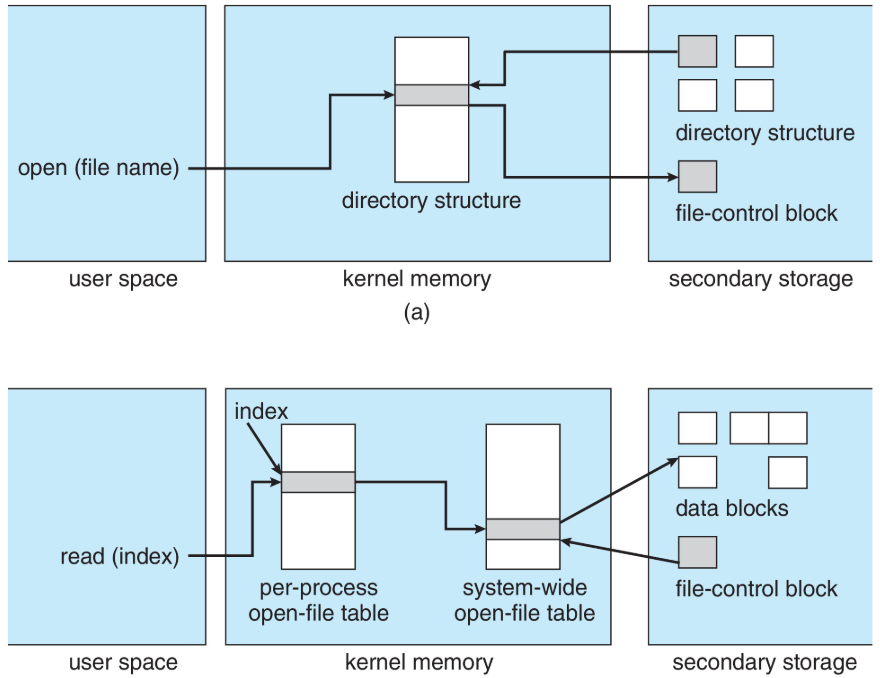
\includegraphics[width=0.5\linewidth]{content/OS_Internals/img/mxfhg.png}
\end{figure}

\newpage
\section{Implementazione delle Directory}

\subsection{Lista Lineare}

Lista lineare di nomi di file con puntatori ai blocchi dati.

\begin{itemize}
    \item Semplice da programmare
    \item Lenta da eseguire: tempo di ricerca lineare; si potrebbe mantenere ordinata alfabeticamente tramite lista collegata o usare un B+ tree
\end{itemize}


\begin{figure}[h!]
    \centering
    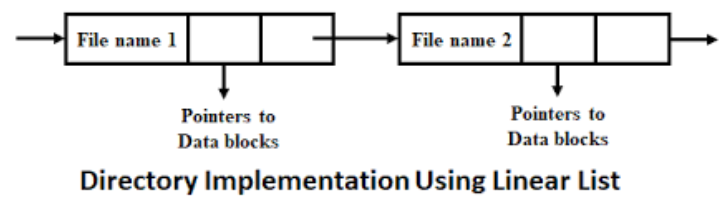
\includegraphics[width=0.5\linewidth]{content/OS_Internals/img/dndsgvg.png}
\end{figure}

\subsection{Tabella Hash}
Tabella Hash - lista lineare con struttura dati hash:
\begin{itemize}
    \item Riduce il tempo di ricerca nella directory
    \item Collisioni - situazioni in cui due nomi di file hanno lo stesso valore hash
    \item Efficiente solo se le voci hanno dimensione fissa, oppure si usa il metodo a catena di overflow
\end{itemize}


\begin{figure}[h!]
    \centering
    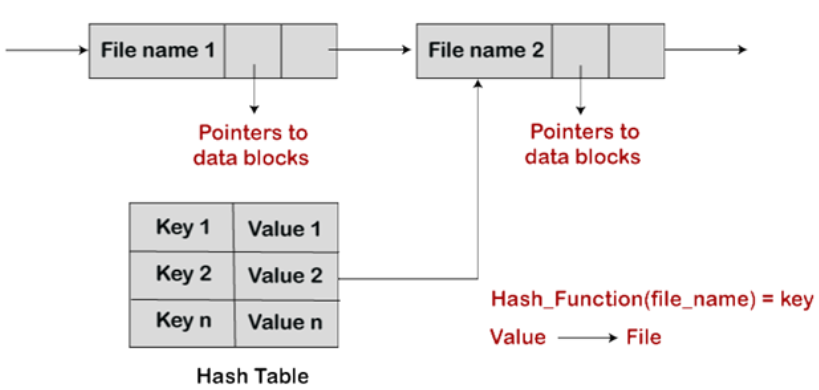
\includegraphics[width=0.5\linewidth]{content/OS_Internals/img/dghgf.png}
\end{figure}

\section{Metodo di Allocazione}

Un metodo di allocazione definisce come i blocchi del disco vengono assegnati ai file:

\begin{itemize}
    \item Contigua
    \item Collegata
    \item Tabella di Allocazione dei File (FAT)
\end{itemize}

\newpage
\subsection{Metodo di Allocazione Contigua}

Ogni file occupa un insieme di blocchi contigui.

\begin{itemize}
    \item Migliori prestazioni nella maggior parte dei casi
    \item Semplice: sono necassari solo la posizione iniziale (numero di blocco) e la lunghezza (numero di blocchi)
    \item I problemi includono:
    \begin{itemize}
    \item Trovare spazio sul disco per un file,
    \item Conoscere la dimensione del file,
    \item Frammentazione esterna nell'HD; necessita di compattazione offline (downtime) o online, detta anche defrag.
    \end{itemize}
\end{itemize}

Mappatura da logico a fisico (dimensione blocco = 512 byte).

\begin{figure}[h!]
    \centering
    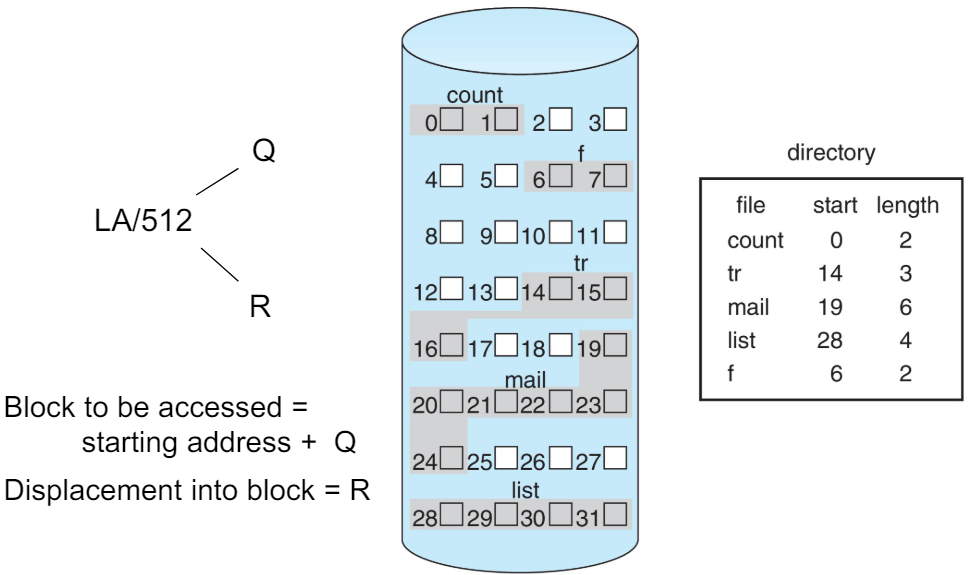
\includegraphics[width=0.6\linewidth]{content/OS_Internals/img/srymkh.png}
\end{figure}


\subsection{Allocazione Collegata}

\begin{itemize}
    \item[] Ogni file è una lista collegata di blocchi
    \item[] Il file termina con un puntatore null
    \item[] Nessuna frammentazione esterna
    \item[] Ogni blocco contiene un puntatore al blocco successivo
    \item[] Nessuna compattazione, nessuna frammentazione esterna
    \item[] Il sistema di gestione dello spazio libero viene chiamato quando è necessario un nuovo blocco
    \item[] Si migliora l'efficienza raggruppando i blocchi in cluster, ma aumenta la frammentazione interna
\end{itemize}
\textbf{Grande problema}: localizzare un blocco richiede molti I/O e seek del disco.

\newpage
Ogni file è una lista collegata di blocchi su disco: i blocchi possono essere sparsi ovunque sul disco

\begin{figure}[h!]
    \centering
    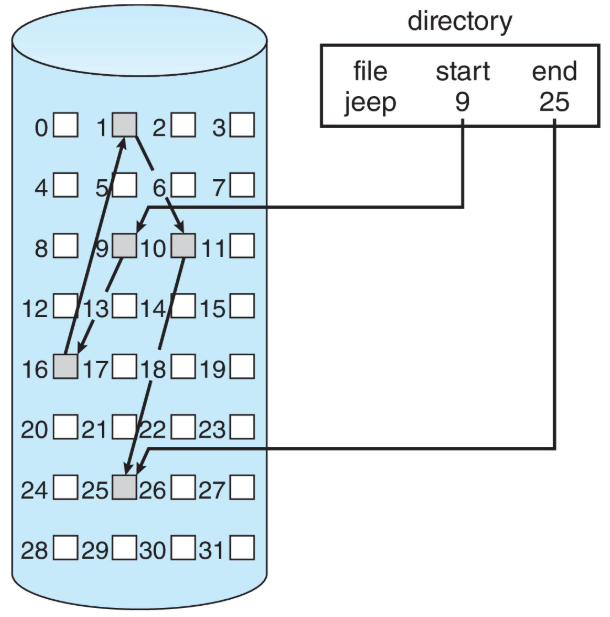
\includegraphics[width=0.4\linewidth]{content/OS_Internals/img/srfymjkgm.png}
\end{figure}

Il blocco da accedere è il $Q^{esimo}$ blocco nella catena collegata di blocchi che rappresenta il file. Spostamento nel blocco = R + 1.

\subsection{Metodo di Allocazione FAT}

L'inizio del volume ha una tabella, indicizzata per numero di blocco. Simile a una lista collegata, ma più veloce su disco e memorizzabile in cache. L'allocazione di nuovi blocchi è semplice.

\begin{figure}[h!]
    \centering
    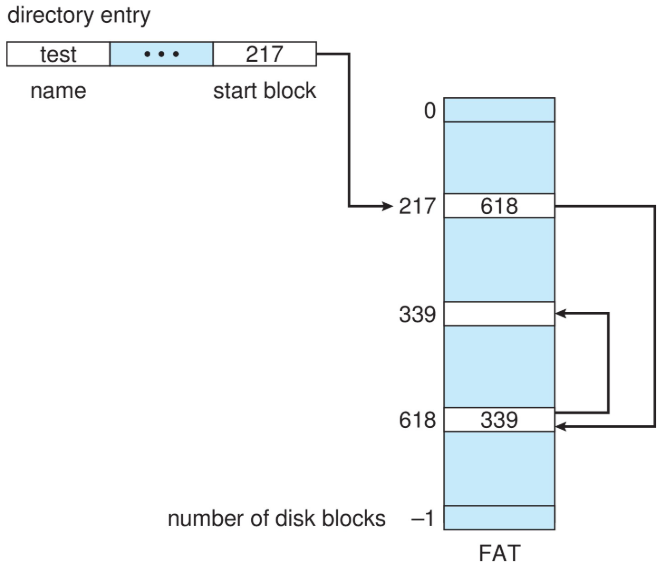
\includegraphics[width=0.5\linewidth]{content/OS_Internals/img/nddgndg.png}
\end{figure}

\newpage
\subsection{Metodo di Allocazione Indicizzata}

Ogni file ha il proprio/i propri blocco/i indice con puntatori ai propri blocchi dati.

\begin{figure}[h!]
    \centering
    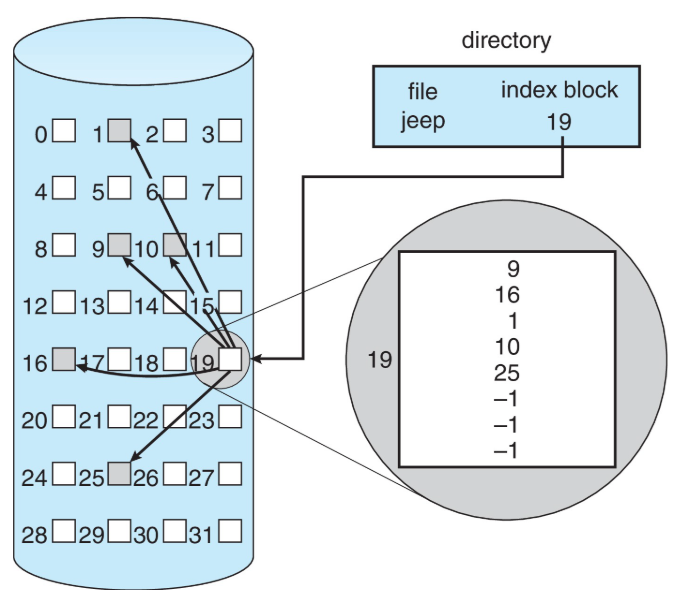
\includegraphics[width=0.5\linewidth]{content/OS_Internals/img/fbfbf.png}
\end{figure}


\subsection{Prestazioni}

Il metodo migliore dipende dal tipo di accesso al file:

\begin{itemize}
    \item L'allocazione contigua è ottima per accesso sequenziale e casuale
    \item L'allocazione collegata è buona per l'accesso sequenziale, non per quello casuale
\end{itemize}

Dichiarare il tipo di accesso alla creazione: scegliere tra contigua o collegata.

L'indicizzata è più complessa: per accedere a un singolo blocco potrebbe essere necessario leggere prima il blocco indice e poi il blocco dati.


\section{Gestione dello Spazio Libero}

Il file system mantiene la \textbf{lista dello spazio libero} per tracciare i blocchi disponibili. Simile alla lista delle pagine libere per la gestione della memoria virtuale.

\textbf{Vettore di bit} o \textbf{bit map} (n blocchi)

\begin{figure}[h!]
    \centering
    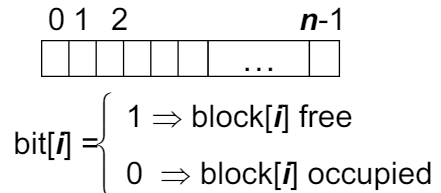
\includegraphics[width=0.45\linewidth]{content/OS_Internals/img/mngaz.png}
\end{figure}

Calcolo del numero di blocco:

\begin{equation*}
    \text{(numero di bit per parola) * (numero di parole con valore 0) + offset del primo bit a 1}
\end{equation*}
Semplice, ma la bit map richiede spazio extra.

\paragraph{Esempio: }



\begin{itemize}
\centering
    \item []dimensione blocco = 4KB = $2^{12}$ byte
    \item[] dimensione disco = $2^{40}$ byte (1 TB)
    \item[] n = $2^{40}$/$2^{12}$ = $2^{28}$ bit (o 32MB)
\end{itemize}

Vantaggio: è facile ottenere spazio per file contigui verificando se ci sono abbastanza blocchi adiacenti liberi

\subsection{Lista Collegata dello Spazio Libero su Disco}

Lista collegata (free list):

\begin{itemize}
    \item \textbf{SVANTAGGIO}: non è facile ottenere spazio contiguo
    \item \textbf{VANTAGGIO}: nessuno spreco. Lista collegata dello spazio libero su disco
\end{itemize}


\begin{figure}[h!]
    \centering
    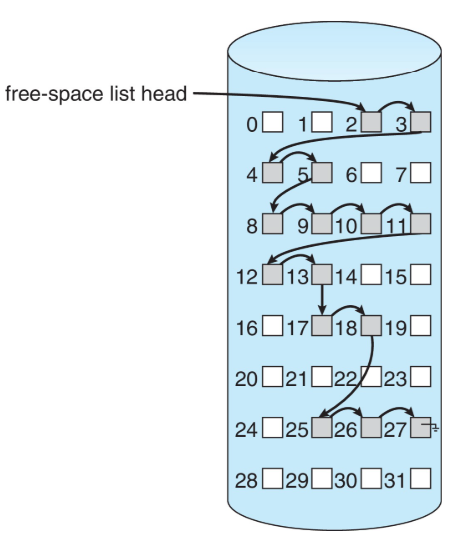
\includegraphics[width=0.4\linewidth]{content/OS_Internals/img/andjfgt.png}
\end{figure}



Non è necessario attraversare l'intera lista (se il numero di blocchi liberi è registrato)

\subsection{Lista Collegata dello Spazio Libero}

\textbf{Raggruppamento:}

\begin{itemize}
    \item Modificare la lista collegata per memorizzare l'indirizzo degli n-1 blocchi liberi successivi nel primo blocco libero, più un puntatore al blocco successivo che contiene puntatori a blocchi liberi (come questo)
    \item I primi n-1 blocchi saranno liberi
    \item L'n-esimo conterrà puntatori agli n-1 blocchi liberi successivi
\end{itemize}

\textbf{Conteggio}

\begin{itemize}
    \item Poiché lo spazio viene spesso usato e liberato in modo contiguo, con allocazione contigua, estensioni o clustering, si mantiene l'indirizzo del primo blocco libero e il conteggio dei blocchi liberi successivi. La lista dello spazio libero contiene quindi voci con indirizzi e conteggi.
    \item Il primo blocco della lista libera conterrà l'indirizzo del blocco libero successivo + il numero di blocchi liberi dopo di esso
    \item Gli altri saranno effettivamente blocchi liberi
\end{itemize}

\section{File System in altri OS}

\subsection{File System di Windows}

\textbf{NTFS}, detto anche New Technology File System, è un file system proprietario con journaling sviluppato da Microsoft. 

A partire da Windows NT 3.1, è il file system predefinito della famiglia Windows NT. Ha soppiantato la File Allocation Table (FAT) come file system preferito su Windows ed è supportato anche da Linux e BSD.


\begin{figure}[h!]
    \centering
    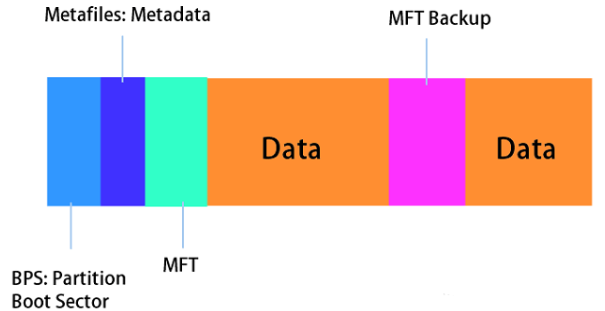
\includegraphics[width=0.5\linewidth]{content/OS_Internals/img/dnfga.png}
\end{figure}
\newpage
\textbf{FAT}, nota anche come File Allocation Table, è un file system sviluppato per personal computer.


Originariamente sviluppata nel 1977 per l'uso su floppy disk, è stata adattata per dischi rigidi e altri dispositivi. È spesso supportata per motivi di compatibilità dai sistemi operativi attuali per PC e da molti dispositivi mobili e sistemi embedded, consentendo l'interscambio di dati tra sistemi diversi.

\paragraph{}
\textbf{FAT32}, successore di FAT16, è stata progettata da Microsoft come nuova versione del file system. FAT32 supporta un numero maggiore di cluster possibili e riutilizza la maggior parte del codice esistente.

\begin{figure}[h!]
    \centering
    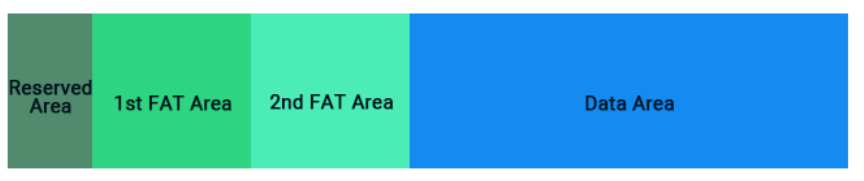
\includegraphics[width=0.55\linewidth]{content/OS_Internals/img/zndfg.png}
    \caption{Struttura del file system FAT32}
\end{figure}


\subsection{Il File System di Apple}

Nel 2017, Apple, Inc., ha rilasciato un nuovo file system per sostituire il suo HFS+ di 30 anni. HFS+ era stato esteso per aggiungere molte nuove funzionalità, ma come di consueto, questo processo ha aggiunto complessità, insieme a righe di codice, e ha reso più difficile aggiungere ulteriori funzionalità. Partire da zero su una pagina bianca consente di avviare una progettazione con le tecnologie e le metodologie attuali e di fornire l'esatto insieme di funzionalità necessarie.

\paragraph{}

\textbf{Apple File System} (APFS) è un buon esempio di tale progettazione. Il suo obiettivo è funzionare su tutti i dispositivi Apple attuali, dall'Apple Watch all'iPhone fino ai Mac. Creare un file system che funzioni su watchOS, iOS, tvOS e macOS è certamente una sfida. APFS è ricco di funzionalità, tra cui puntatori a 64 bit, cloni per file e directory, snapshot, condivisione dello spazio, calcolo rapido della dimensione delle directory, operazioni atomiche di salvataggio sicuro, design copy-on-write, cifratura (mono- e multi-chiave) e I/O coalescing. Supporta sia l'archiviazione NVM che HDD.

\paragraph{}

Molte di queste funzionalità sono state già discusse, ma ci sono alcuni nuovi concetti che vale la pena esplorare. La \textbf{condivisione dello spazio} è una funzionalità simile a ZFS in cui lo storage è disponibile come uno o più grandi spazi liberi (\textbf{container}) da cui i file system possono attingere allocazioni (permettendo ai volumi APFS di crescere e ridursi).

Il \textbf{calcolo rapido della dimensione delle directory} fornisce un aggiornamento rapido dello spazio usato. L'\textbf{atomic safe-save} è una primitiva (disponibile tramite API, non tramite comandi del file system) che esegue ridenominazioni di file, bundle di file e directory come operazioni atomiche singole. L'I/O coalescing è un'ottimizzazione per i dispositivi NVM in cui più piccole scritture vengono raggruppate in una grande scrittura per ottimizzare le prestazioni di scrittura.
\paragraph{}
Apple ha scelto di non implementare RAID come parte del nuovo APFS, dipendendo invece dal meccanismo Apple RAID volume per il RAID software. APFS è anche compatibile con HFS+, consentendo una facile conversione delle installazioni esistenti.
